\documentclass[11pt]{article}
\usepackage[a4paper, total={6.8in, 9.25in}]{geometry}
\usepackage{graphicx}
\graphicspath{ {./assets/images/output/} }
\usepackage{caption}
\usepackage[english]{babel}
\usepackage{titling}
\usepackage{float}
\usepackage{amsmath}
\usepackage{minted}
\usepackage{multicol}
\usepackage{array}
\usepackage{setspace}
\usepackage{placeins}
\usepackage{tabularx}
\usepackage{booktabs}

% \usepackage{lipsum}

\title{Study of Static Routing Configuration Using VLSM Technique and Simulation}
\author{}
\date{}

\pagenumbering{gobble}
\begin{document}
\input{cn_cover.tex}

\pagebreak

\tableofcontents

\pagebreak
\pagenumbering{arabic}
\maketitle

% --- Theory and Introduction ---
\section{Theory and Introduction}
Variable Length Subnet Mask (VLSM) is a method used in IP network design to create subnets with varying subnet masks. By allowing different subnet sizes, VLSM enables network administrators to allocate IP addresses more efficiently, using smaller subnet masks for subnets with fewer hosts and larger masks for those with more hosts.

Unlike traditional subnetting (Classful routing), where a fixed subnet mask is applied to all subnets across a network, VLSM provides greater flexibility, drastically reducing IP address waste \cite{tanenbaum2021}. It is commonly used in modern networks to optimize IP address usage. Conceptually, VLSM can be described as the process of further subnetting an already existing subnet. In this experiment, a single Class C network block (192.168.1.0/24) was partitioned using VLSM to accommodate four separate Local Area Networks (LANs) and three Wide Area Network (WAN) links using static routing.

% --- Methodology ---
\section{Methodology}
The experiment was conducted using Cisco Packet Tracer (Version 9.0). The static routing network was established through the following systematic steps:

\begin{itemize}
    \item \textbf{VLSM Calculation:} A VLSM allocation table was prepared based on the specific host requirements of the network topology to carve multiple subnets from the 192.168.1.0/24 block.
    \item \textbf{Topology Construction:} The network was designed utilizing three routers. Four distinct LANs were created: Router 0 hosted a 30-host network, Router 1 hosted a 14-host network, and Router 2 hosted two smaller networks for varying host capacities.
    \item \textbf{Interface Configuration:} High-speed serial links were configured between the routers. Point-to-point connections utilized /30 subnet masks to maximize efficiency.
    \item \textbf{Addressing:} Each PC, switch, and router interface was assigned its specific IPv4 address, subnet mask, and default gateway according to the simulated VLSM table.
    \item \textbf{Static Routing:} The global configuration mode on each router was accessed to manually input static routes. The destination network address, VLSM subnet mask, and Next-Hop IP address were explicitly defined.
    \item \textbf{Verification:} The \texttt{show ip route} command was utilized to verify the routing tables. End-to-end connectivity was tested by sending ICMP messages between hosts on different subnets.
\end{itemize}

% --- Results ---
\section{Results}
The network was successfully simulated. Table 1 reflects the VLSM subnets as configured in the simulation environment, and Table 2 outlines the device interfaces.

\begin{table}[H]
    \centering
    \caption{Simulated VLSM Subnet Allocation Table}
    \resizebox{\textwidth}{!}{%
        \begin{tabular}{@{}llllll@{}}
            \toprule
            \textbf{Segment}     & \textbf{Network Address} & \textbf{CIDR} & \textbf{Subnet Mask} & \textbf{Usable Host Range}   & \textbf{Broadcast Address} \\ \midrule
            LAN 0 (Router 0)     & 192.168.1.0              & /27           & 255.255.255.224      & 192.168.1.1 -- 192.168.1.30  & 192.168.1.31               \\
            LAN 1 (Router 1)     & 192.168.1.32             & /28           & 255.255.255.240      & 192.168.1.33 -- 192.168.1.46 & 192.168.1.47               \\
            LAN 2 (Router 2 - A) & 192.168.1.48             & /29           & 255.255.255.248      & 192.168.1.49 -- 192.168.1.54 & 192.168.1.55               \\
            LAN 3 (Router 2 - B) & 192.168.1.56             & /29           & 255.255.255.248      & 192.168.1.57 -- 192.168.1.62 & 192.168.1.63               \\
            WAN 1 (Router 0 - 1) & 192.168.1.56             & /30           & 255.255.255.252      & 192.168.1.57 -- 192.168.1.58 & 192.168.1.59               \\
            WAN 2 (Router 1 - 2) & 192.168.1.60             & /30           & 255.255.255.252      & 192.168.1.61 -- 192.168.1.62 & 192.168.1.63               \\
            WAN 3 (Router 2 - 0) & 192.168.1.64             & /30           & 255.255.255.252      & 192.168.1.65 -- 192.168.1.66 & 192.168.1.67               \\ \bottomrule
        \end{tabular}%
    }
\end{table}

\begin{table}[H]
    \centering
    \caption{Device IPv4 Addressing Summary}
    \resizebox{0.9\textwidth}{!}{%
        \begin{tabular}{@{}lllll@{}}
            \toprule
            \textbf{Device} & \textbf{Interface} & \textbf{IPv4 Address} & \textbf{Subnet Mask} & \textbf{Default Gateway} \\ \midrule
            Router 0        & Fa0/0              & 192.168.1.1           & 255.255.255.224      & N/A                      \\
            Router 0        & Se2/0              & 192.168.1.57          & 255.255.255.252      & N/A                      \\
            Router 0        & Se3/0              & 192.168.1.66          & 255.255.255.252      & N/A                      \\
            Router 1        & Fa0/0              & 192.168.1.33          & 255.255.255.240      & N/A                      \\
            Router 1        & Se2/0              & 192.168.1.58          & 255.255.255.252      & N/A                      \\
            Router 2        & Fa0/0              & 192.168.1.49          & 255.255.255.248      & N/A                      \\
            Router 2        & Fa1/0              & 192.168.1.57          & 255.255.255.248      & N/A                      \\
            PC 11 (A)       & NIC                & 192.168.1.2           & 255.255.255.224      & 192.168.1.1              \\
            PC 21 (B)       & NIC                & 192.168.1.34          & 255.255.255.240      & 192.168.1.33             \\
            PC 31 (C)       & NIC                & 192.168.1.54          & 255.255.255.248      & 192.168.1.49             \\
            PC 41 (D)       & NIC                & 192.168.1.58          & 255.255.255.248      & 192.168.1.57             \\ \bottomrule
        \end{tabular}%
    }
\end{table}

\subsection{Configuration Notes}
The addressing plan was applied from the largest subnet to the smallest subnet to minimize address waste and avoid fragmentation. Each router was configured with an IP address on its LAN-facing interface and appropriate next-hop routes for remote LANs. The serial links were assigned /30 masks because each point-to-point connection requires only two usable host addresses.

\subsection{Static Route Summary}
To enable inter-network communication, static routes were manually added on each router so that traffic could reach all remote LAN segments through the correct intermediate router. This configuration ensured that packets followed the intended path across the three-router topology and allowed successful ICMP verification between hosts in different subnets.

\begin{figure}[H]
    \centering
    
\includegraphics[width=\textwidth]{network.png}
    \caption{Multi-Router Topology with VLSM Implementation}
\end{figure}

\begin{figure}[H]
    \centering
    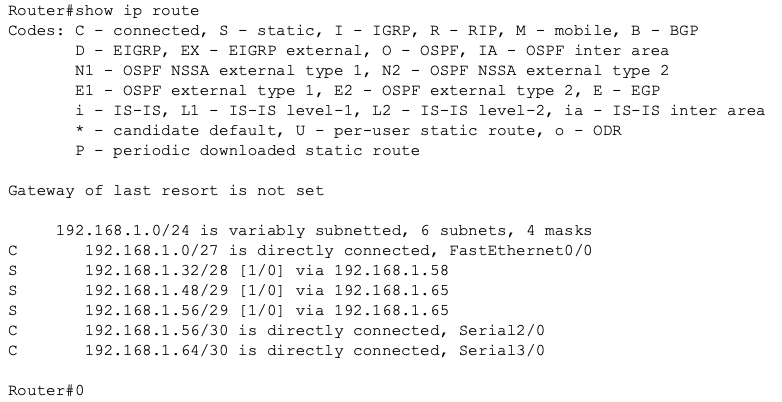
\includegraphics[width=0.8\textwidth]{router0_route.png}
    \caption{Router 0 CLI: Routing Table Output displaying "Variably Subnetted" feature}
\end{figure}

\begin{figure}[H]
    \centering
    \begin{minipage}{0.48\textwidth}
        \centering
        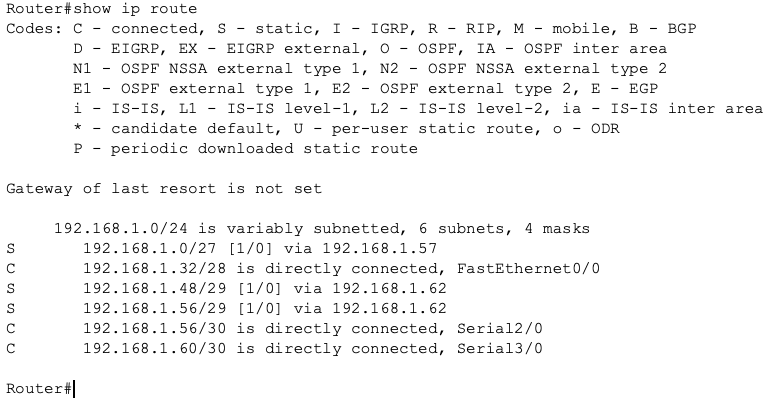
\includegraphics[width=\linewidth]{router1_route.png}
        \caption{Router 1 Routing Table}
    \end{minipage}\hfill
    \begin{minipage}{0.48\textwidth}
        \centering
        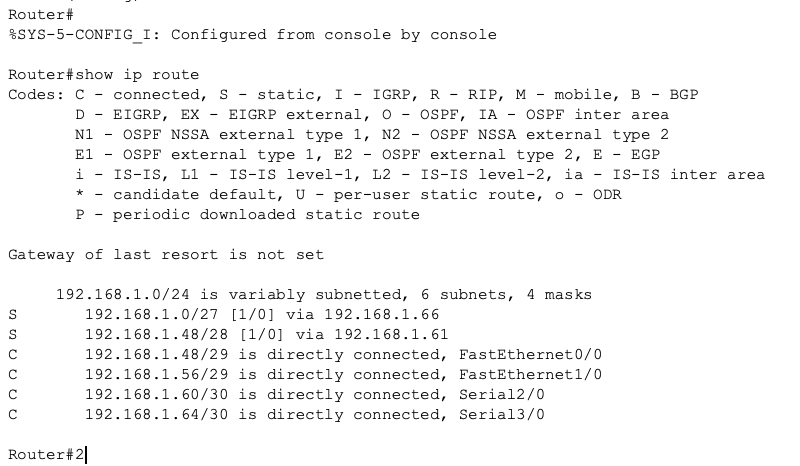
\includegraphics[width=\linewidth]{router2_route.png}
        \caption{Router 2 Routing Table}
    \end{minipage}
\end{figure}

\begin{figure}[H]
    \centering
    
\includegraphics[width=0.85\textwidth]{ping.png}
    \caption{Verification of End-to-End Connectivity between distinct VLSM Subnets}
\end{figure}

% --- Discussion ---
\section{Discussion}
The implementation of VLSM drastically improved the IP address efficiency of the network. As displayed in the \texttt{show ip route} output for Router 0 (Figure 2), Cisco IOS explicitly recognized the single Class C block as being "variably subnetted" into 6 subnets using 4 different masks. Utilizing /30 masks on the serial links was highly effective, conserving address space by providing exactly two IP addresses per point-to-point connection.

During the configuration analysis, two notable routing behaviors were observed that highlight the complexities of static VLSM environments:
\begin{enumerate}
    \item \textbf{Subnet Overlap \& Longest Prefix Match:} Table 1 indicates an overlap between LAN 3 (192.168.1.56/29) and WAN 1 (192.168.1.56/30). Because the /30 mask is longer than the /29 mask, Router 0 forwarded traffic destined for PC 41 via the WAN link to Router 1, which then successfully relayed it to Router 2. This demonstrated the "Longest Prefix Match" rule in routing architecture, allowing the ICMP packets to successfully reach their destination (Figure 5) despite the overlap.
    \item \textbf{Configuration Discrepancy:} The routing table for Router 2 (Figure 4) revealed a static route entry of \texttt{192.168.1.48/28 via 192.168.1.61}. This entry was likely intended to route traffic to the 192.168.1.32/28 network. Consequently, ICMP requests initiated from Router 2 to Router 1 would fail because the static route was pointing to an incorrect block.
\end{enumerate}

These observations underscore that while VLSM provides unparalleled addressing efficiency, it requires meticulous planning and precise static route implementation to prevent logical overlap and blackhole routing.

% --- Conclusion ---
\section{Conclusion}
The study and simulation of static routing utilizing the Variable Length Subnet Mask (VLSM) technique were successfully executed. The experiment confirmed that routers can seamlessly forward traffic between networks of varying sizes—such as /27, /28, and /29 subnets—within a single parent IP block. The analysis of the routing tables proved that VLSM is a fundamental tool for network administrators to conserve IPv4 address space, though it demands careful schematic planning to avoid overlapping ranges in static environments.

\bibliographystyle{IEEEtran}
\renewcommand{\bibname}{References}
\addcontentsline{toc}{section}{References}
\bibliography{ref}

\end{document}
